\documentclass[12pt]{article}

\usepackage[brazil]{babel}
\usepackage[utf8]{inputenc}
\usepackage{amsmath}
\usepackage{amsfonts}
\usepackage{amssymb}
\usepackage{indentfirst}
\usepackage{color}
\usepackage{mathrsfs}
\usepackage{pgfplots}
\usepackage{hyperref}
\usepackage{fancyhdr}
\usepackage[export]{adjustbox}


\fancypagestyle{plain}{%
	\fancyfoot{}%
	\fancyhead{}%
}
\fancyhead{}
\fancyhead[L]{\leftmark}
\fancyfoot{}
\fancyfoot[L]{{\footnotesize  COMPPET - Programa de Educação Tutorial}}
\fancyfoot[C]{\hspace{3.0cm}\thepage}
\fancyfoot[R]{{\footnotesize Curso de Inclusão Digital}}
\begin{document}
\pagestyle{fancy}
	
\tableofcontents
{\let\thefootnote\relax\footnotetext{* \textit{COMPPET - UFU, Universidade Federal de Uberlândia, Minas Gerais, Brasil}}}

{\let\thefootnote\relax\footnotetext{* \textit{PETMEC - UFU, Universidade Federal de Uberlândia, Minas Gerais, Brasil}}}

\newpage

\section{Introdução}
\paragraph{} oi tudo bem  ? a introdução vem aki 

\section{Ligando e Desligando o Computador}
\subsection{Ligando o Computador} 

\paragraph{} Para ligar o computador, devemos seguir os seguintes passos: \\
\begin{itemize}
	
	\item Verificar os cabos de energia do computador;
	
	\item Verificar se a voltagem está correta (110 volts ou 220 volts);
	
	\item Verificar se existe um estabilizador \href{Fig:estabilizador} de voltagem, e se existir, verificar a voltagem da 
	dele (110 v ou 220 v). Essa voltagem deve ser compatível com a voltagem utilizada na sua casa, ou no trabalho;
	
	\item Quando todos os cabos estiverem conectados, ligar o estabilizador. Ele possui um botão Liga/Desliga de acesso e identificação simples;

	\item Ligar o PC através do botão Liga/Desliga, localizado no gabinete;
	
	\item Aguardar os procedimentos de inicialização do computador; 
	
	\item Informar senha e nome do usuário, caso existam e quando for solicitado.


\end{itemize}

\subsection{Desligando o Computador}
\paragraph{} O procedimento de desligar o computador é muito importante para preservar o equipamento e as informações armazenadas nele, portanto, é importantíssimo acostumar-se a seguir o procedimento de desligar:\\

\begin{itemize}
	\item Clicar no botão Iniciar;
	
	\item Clicar na opção Desligar; 
	
	\item Esperar o computador desligar automaticamente; 
	
	\item Desligar o estabilizador através do botão Liga/Desliga do estabilizador.
\end{itemize}

\begin{figure}[!hb]
	\centering	
	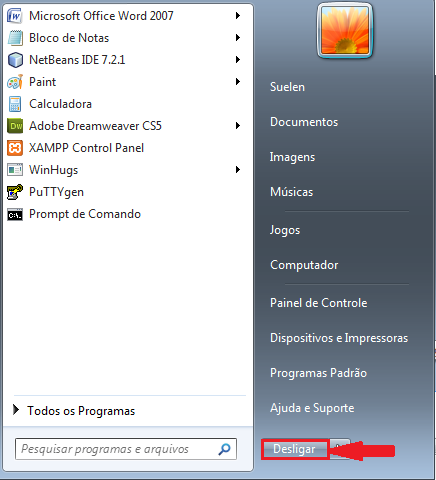
\includegraphics{Figures/desligando.png}
	\caption{Desligando o Computador}
	\label{fig:desligando}
\end{figure}

\newpage

\section{O windows 7}
\subsection{Área de Trabalho (Desktop)}

O Windows é o sistema operacional criado pela Microsoft Corporation® que tem como principal característica o uso de janelas para facilitar a utilização dos diversos aplicativos existentes no sistema. Antes do conceito de janelas, os sistemas operacionais eram utilizados em modo de texto. Ainda existem sistemas que se utilizam desse recurso, como é o caso de algumas versões do Linux.

No meio computacional, uma área de trabalho consiste de um ambiente gráfico adequado às necessidades de cada usuário. A área de trabalho permite a colocação de ícones dos programas mais utilizados, facilitando a vida do usuário.\\

\begin{figure}[!hb]
	\centering
	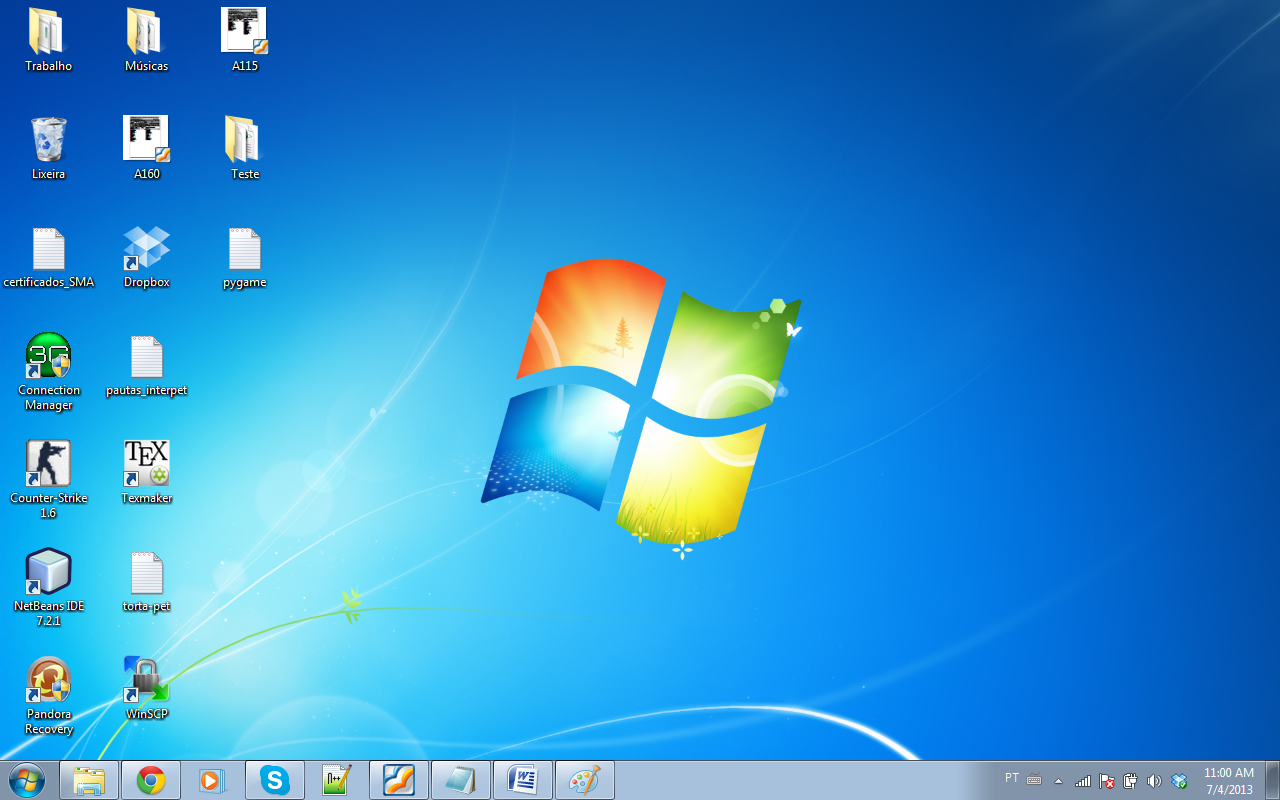
\includegraphics[scale=0.3]{Figures/desktop}
	\caption{Desktop}
	\label{fig:desktop}
\end{figure}


\subsection{Ícones}
	Os ícones na área de trabalho servem de atalhos para os programas mais utilizados.	
	Organizar os ícones da área de trabalho é uma tarefa semelhante a organizar as janelas. Em uma parte vazia do Desktop, clique no botão direito do mouse e selecione a opção: 

	Classificar por $->$ Nome
	
	 \hspace{3.6cm}Tamanho
	 
	 \hspace{3.6cm}Tipo de item
	 
	 \hspace{3.6cm}Data de modificação.
	
	 Existe uma outra opção chamada Exibir. Clicando nela com o botão esquerdo do mouse você pode Organizar ícones automaticamente. Uma outra opção é soltar o ícone em qualquer parte da área de trabalho.
	
	
	\begin{figure}[!htbp]
		\centering
		\begin{minipage}[b]{0.45\textwidth}
			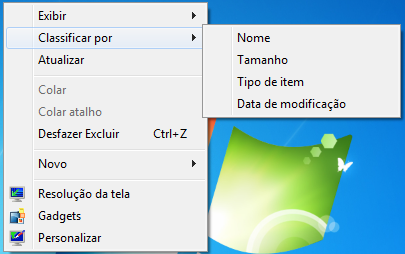
\includegraphics[width=\textwidth]{Figures/icone1}
			\caption{Classificar por}
			\label{fig:classificar por}
		\end{minipage}
		\hfill
		\begin{minipage}[b]{0.45\textwidth}
			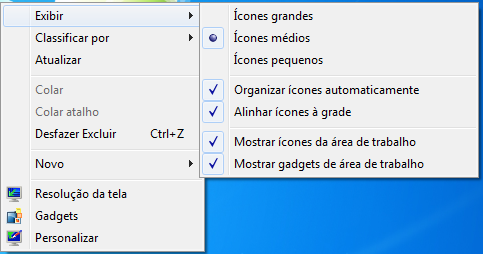
\includegraphics[width=\textwidth]{Figures/icone2}
			\caption{Exibir}
			\label{fig:exibir}
		\end{minipage}
	\end{figure}

\subsection{Barra de Tarefas}

	É uma barra de ferramentas gráficas usada para controlar a execução dos programas dispostos em janelas, classificando-as como ativa ou inativa. Tem como principal componente o botão iniciar.
	
	É subdividida em:
	
\begin{itemize}
	\item Menu Iniciar – nele estão organizados todos os programas do computador para um acesso imediato;

	\item Barra de Inicialização Rápida – podem ser colocados nesta área os programas mais utilizados pelo usuário;

	\item Janela Ativa ou Inativa – nesta área aparecem todas as janelas que estão ativas ou inativas (os programas que estão em execução são mostrados);

	\item Área de Notificação – os programas que estão sendo controlados pelo sistema aparecem nesta área, inclusive o relógio.
	
\end{itemize}
	
		\begin{figure}[!hb]
			%\centering
			
\includegraphics[width=1\textwidth,left]{Figures/menuiniciar}
			\label{fig:menu iniciar}
		
		\end{figure}	
	  {\vspace{-0.8cm}\hspace{-0.6cm}\huge{$\Downarrow$}}     {\vspace{-0.8cm}\hspace{3.6cm}\huge{$\Downarrow$}}
	  {\vspace{-0.8cm}\hspace{7.6cm}\huge{$\Downarrow$}}\\
	  \bigskip
	  
	  \vspace{1cm}
	  \hspace{-0.6cm}{\small Iniciar } \hspace{1cm}{\tiny Barra de Inicialização Rápida e Janelas Ativas e Inativas}
	  \hspace{1.2cm}{\small Área de Notificação}
	  \newpage
  
  \subsection{Relógio/Calendário}
	
	O relógio está localizado na extrema direita da barra de tarefas. Para fazer a visualização da data, basta clicar em cima da hora. Para fazer correção de hora e/ou data, basta clicar em {\bf Alterar configurações de data e hora}. 
	
	\begin{figure}[!hb]
		\centering
		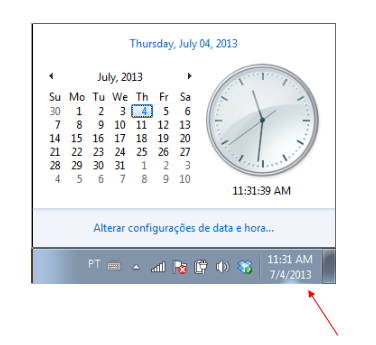
\includegraphics[scale=0.9]{Figures/relogio}
		\caption{Relógio do Windows 7}
		\label{fig:relogio}
		
	\end{figure}
	
	Após serem feitas as modificações de data e hora deve-se clicar no botão {\bf OK} para que as atualizações sejam salvas
	
	\begin{figure}[!h]
		\centering
		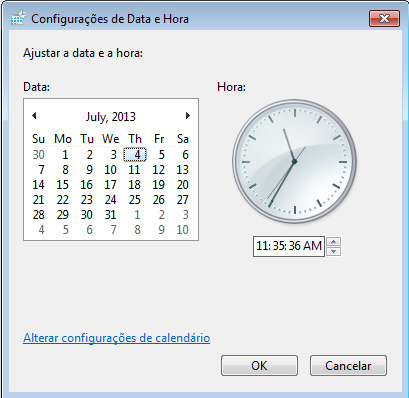
\includegraphics[scale=0.9]{Figures/relogio2}
		\caption{Calendário do Windows 7}
		\label{fig:calendario}
		
	\end{figure}
	
	\newpage
	\subsection{Menu Iniciar}
	
	Através do menu Iniciar podemos acessar os diversos recursos disponíveis em nosso computador. Nele estão contidos todos os programas instalados no computador, diversas ferramentas de manutenção do sistema e ferramentas úteis como a calculadora, bloco de notas e o Google Chrome \footnote{O naveggador padrão é o Internet Explorer, no entanto, o Chrome apresenta melhor desempenho.} que é o programa de navegação na internet . Ao se clicar neste, abrirá no computador uma janela semelhante a da figura abaixo:
	
	
	\begin{figure}[!h]
		\centering
		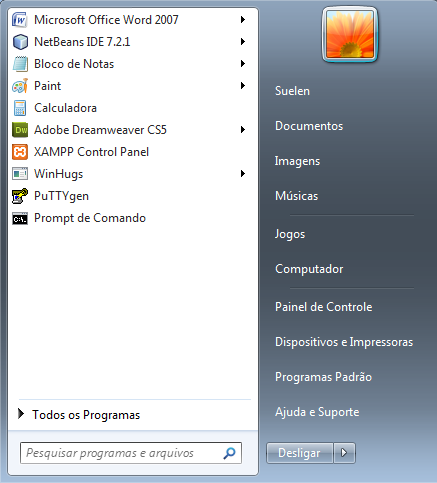
\includegraphics[scale=0.9]{Figures/iniciar}
		\caption{Iniciar}
		\label{fig:iniciar}
		
	\end{figure}
	\newpage
	\begin{itemize}
	\item Na coluna da esquerda, fica a lista dos programas usados mais recentemente.

	\item Todos os programas – Nele você encontra os ícones de todos os programas instalados assim como as ferramentas de administração do sistema.
	
	\item Documentos – Aqui podem ser guardados todos os documentos produzidos no computador.
	
	\item Imagens – É uma pasta para armazenagem de imagens.
	
	\item Músicas – É uma pasta que contém ou podem ser armazenados diversos formatos de áudio.
	
	\item Jogos – Aqui encontra-se todos os jogos disponíveis do computador.
	
	\item Computador – Aqui você pode ter acesso às pastas do sistema operacional.
	
	\item Painel de Controle – Contém opções de configuração do computador.
	
	\item Dispositivos e Impressoras – Aqui se encontram as impressoras e aparelhos de fax instalados no computador.
	
	\item Programas Padrão – Aqui pode-se definir os programas que o Windows usa por padrão.
	
	\item Ajuda e suporte – Tire suas dúvidas e encontre soluções para diversos problemas que possam aparecer no sistema operacional.
	
	\item Pesquisar Programas e Arquivos – Localizar imagens, pastas e arquivos.
	
	\item Desligar – Opções: Trocar usuário, Fazer logoff, Bloquear, Reiniciar, Suspender e Hibernar.
	\end{itemize}
	
	\section{Interface}	
	Seguem questões relacionadas à interface do computador
	
	\subsection{Janelas}
	Existem algumas ferramentas que facilitam a manipulação das janelas que são abertas no ambiente Windows.
	
	\subsection{Barra de Rolagem}
	Esta barra serve para mover ambientes gráficos dentro das janelas. Podem estar na posição vertical ou horizontal.
	
	\subsection{Redimensionando uma janela}
	Para redimensionar uma janela, leve o ponteiro do mouse até a quina da janela e arraste até o tamanho desejado.
	
	\begin{figure}[!h]
		\centering
		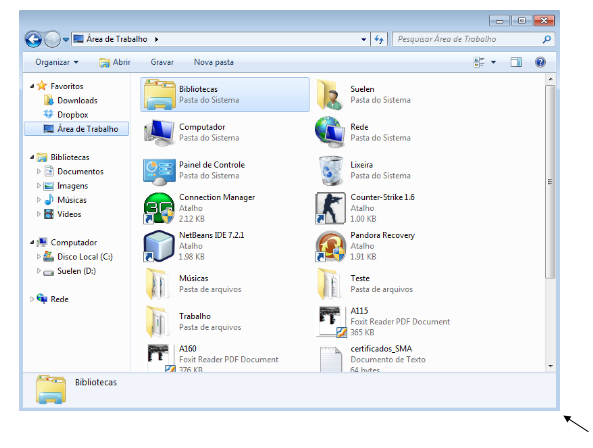
\includegraphics[scale=0.5]{Figures/red_janela}
		\caption{Leve o ponteiro do mouse até a área apontada pela seta como ilustrado acima}
		\label{fig:redimensionando janela}
		
	\end{figure}
	
	
	\section{Botões}
	
	
	\begin{figure}[!h]
			
\includegraphics[scale=0.5]{Figures/minimizar}
			\label{fig:min }
	\end{figure}
	
	\vspace{-1cm}{\bf Botão Minimizar}: reduz ou minimiza uma janela a um botão da barra de tarefas do Windows (seu programa se torna um ícone da barra de tarefas).
	
	\begin{figure}[!h]
		
\includegraphics[scale=0.5]{Figures/maximizar}
		\label{fig:max}
	\end{figure}
	
	\vspace{-1cm}{\bf Botão Maximizar}: aumenta ou maximiza uma janela (deixa a janela do tamanho da tela do computador).
	
	\begin{figure}[!h]
		
\includegraphics[scale=0.5]{Figures/restaurar}
		\label{fig:restaurar}
	\end{figure}
	
	\vspace{-1cm}{\bf Botão Restaurar}: restaura uma janela para o seu tamanho ou posição anterior.
	
	\begin{figure}[!h]
		
\includegraphics[scale=0.5]{Figures/fechar}
		\label{fig:fechar}
	\end{figure}
	
	\vspace{-1cm}{\bf Botão Fechar}: fecha um programa ou janela ativa. Caso um arquivo aberto não tenha sido salvo ou contenha alterações não salvas, você será solicitado a salvar ou não o arquivo antes de fechá-lo.
	
	
	\section{Movendo uma Janela}
	
	
	
	
	
	
\end{document}